\documentclass[t]{beamer}

\usetheme{Air}
\usepackage{graphics}
\usepackage{graphicx}
\graphicspath{{../images/}{../diagrams/}{.}}
%\usepackage{caption}
\usepackage{amsthm}
%\usepackage{thumbpdf}
\usepackage{wasysym}
\usepackage{ucs}
\usepackage[utf8]{inputenc}
\usepackage{pgf}
\usepackage{verbatim}
\usepackage{tikz}
\usepackage{pgfmath}
\usetikzlibrary{calc}
\usetikzlibrary{backgrounds}
\usetikzlibrary{arrows}
\usetikzlibrary{shapes.arrows}
\usetikzlibrary{shapes.geometric}
\usetikzlibrary{decorations.markings}
\usetikzlibrary{positioning}
\usetikzlibrary{fit,chains}
\usepackage{natbib}
\usepackage{wasysym}
\usepackage{soul} 
\bibliographystyle{apalike}  

%\usepackage[bottom, ragged]{footmisc}
%\usepackage{pstricks}
%\newpsobject{psid}{psline}{linestyle=dotted,dotsep=1pt}
%\newpsobject{pspsi}{psline}{doubleline=true}
%\newpsobject{pssigma}{psline}{linewidth=1.5pt}

%\usepackage{pgfpages}
%\setbeamertemplate{note page}[plain]
%\setbeameroption{show notes on second screen=right}
%http://tex.stackexchange.com/questions/21777/is-there-a-nice-solution-to-get-a-presenter-mode-for-latex-presentations

\newcommand{\beq}{\begin{equation}}
\newcommand{\eeq}{\end{equation}}
\newcommand{\beqa}{\begin{eqnarray}}
\newcommand{\eeqa}{\end{eqnarray}}
\newcommand{\bi}{\begin{itemize}}
\newcommand{\ei}{\end{itemize}}
\newcommand{\ket} [1] {\vert #1 \rangle}
\newcommand{\bra} [1] {\langle #1 \vert}
\newcommand{\braket}[2]{\langle #1 | #2 \rangle}
\newcommand{\ev}[1]{\langle #1 \rangle}
\newcommand{\vbra}[1]{\left ( #1 \right |}
\newcommand{\vket}[1]{\left |#1 \right )}
\newcommand{\vbraket}[2]{\left ( #1 \middle |#2 \right )} 
\newcommand{\braopket}[3]{\left \langle #1 \middle |#2 \middle | #3 \right \rangle} 
\newcommand{\vbraopket}[3]{\left ( #1 \middle |#2 \middle | #3 \right )} 

%\newcommand<>{\highlighton}[1]{%
%  \alt#2{\structure{#1}}{{#1}}
%}

\newcommand{\icon}[1]{\pgfimage[height=1em]{#1}}

\usepackage{empheq}

\newlength\mytemplen
\newsavebox\mytempbox

\makeatletter
\newcommand\mybluebox{%
    \@ifnextchar[%]
       {\@mybluebox}%
       {\@mybluebox[0pt]}}

\def\@mybluebox[#1]{%
    \@ifnextchar[%]
       {\@@mybluebox[#1]}%
       {\@@mybluebox[#1][0pt]}}

\def\@@mybluebox[#1][#2]#3{
    \sbox\mytempbox{#3}%
    \mytemplen\ht\mytempbox
    \advance\mytemplen #1\relax
    \ht\mytempbox\mytemplen
    \mytemplen\dp\mytempbox
    \advance\mytemplen #2\relax
    \dp\mytempbox\mytemplen
    \fcolorbox{airlightblue}{white}{\hspace{1em}\usebox{\mytempbox}\hspace{1em}}}

\makeatother

\tikzset{peps/.style={circle=2pt,draw=black!100,fill=green!50,inner sep=3pt}}
\tikzset{bpeps/.style={circle=2pt,draw=black!100,thick,fill=green!50,inner sep=3pt}}
\tikzset{gamma/.style={circle=2pt,draw=black!100,fill=blue!20,inner sep=3pt}}
\tikzset{lambda/.style={rectangle,rotate=45,draw=black!100,fill=orange!50,inner sep=4pt}}
\tikzset{operator/.style={circle=2pt,draw=black!100,fill=orange!80,inner sep=3pt}}
\tikzset{cdot/.style={circle=2pt,draw=black!100,fill=white,inner sep=1pt}}
\tikzset{bg/.style={rounded corners,thin,fill=blue!10}}
\tikzset{inv/.style={opacity=0}}
\tikzset{spin/.style={circle=2pt,draw=black!100,fill=orange!80,inner sep=3pt}}
\tikzset{unitbox/.style={fill=black!3,rounded corners}}
\tikzset{corner/.style={rectangle=10pt,fill=blue!50,draw=black}}
\tikzset{side/.style={rectangle=6pt,fill=blue!20,draw=black}}
\tikzset{cside/.style={circle=6pt,fill=blue!20,draw=black}}
\tikzset{swapg/.style={circle=1pt,draw=black,fill=black!80,inner sep=1pt}}

\tikzset{base/.style={circle=2pt,fill=orange!80,draw=black}}
\tikzset{det/.style={circle=2pt,fill=blue!20,draw=black,inner sep=4pt}}
\tikzset{iso/.style={circle=2pt,fill=red!20,draw=black,inner sep=4pt}}
\tikzset{top/.style={circle=2pt,fill=black!20,draw=black,inner sep=4pt}}
\tikzset{siso/.style={circle=1pt,fill=red!20,draw=black,inner sep=1pt}}

%Brayden's
\tikzset{GHZ/.style={circle=2pt,fill=black!80,draw=black,inner sep=2pt}}
\tikzset{X/.style={circle=2pt,fill=black!80,text=white,font=\footnotesize, draw=black,inner sep=1pt}}
\tikzset{W/.style={circle=2pt,fill=black!20,draw=black,double,inner sep=2pt}}
\tikzset{eli/.style={ellipse, rotate=0, draw=black, fill=gray!20}}

%http://tex.stackexchange.com/questions/199683/how-to-plot-quantum-logical-gates-with-tikz
\tikzset{
cross/.style={path picture={ 
            \draw[thick,black](path picture bounding box.north) -- (path picture bounding                  box.south) (path picture bounding box.west) -- (path picture bounding                      box.east);
            }},
crossx/.style={path picture={ 
            \draw[thick,black,inner sep=0pt]
                (path picture bounding box.south east) -- (path picture bounding box.north west) (path picture bounding box.south west) -- (path picture bounding box.north east);
            }},
circlewc/.style={circle=2pt,draw, crossx}
}
%\newtheorem{LSM}{{\em Theorem: Lieb, Schultz, Mattis (1961)}}
%\newtheorem{Oshikawa}{{\em Extension: Oshikawa (1999)}}

\pdfinfo
{
  /Title       (Entanglement in Featureless Mott Insulators)
  /Creator     (TeX)
  /Author      (Brayden Ware)
}


\title{Entanglement in Featureless Mott Insulators}
%\subtitle{}
\author{Brayden Ware \inst{1} \newline \newline \and Itamar Kimchi \inst{2} \and Siddarth Parameswaran \inst{3} \and Bela Bauer \inst{4}}
\institute[shortinst]{\inst{1} UC Santa Barbara \quad  %
                      \inst{2} UC Berkeley \quad %
                      \inst{3} UC Irvine \quad %
                      \inst{4} Microsoft Station Q}
\date{March 6th 2014}

%\includeonly{slides/LSM1}
\begin{document}

\frame{\titlepage}


%%%%%%%%%%%%%%%%%%%%%%%%%%%%%%%%%%%%%%%%%
%%%%%%%%%% Pre-outline section %%%%%%%%%%
%%%%%%%%%%%%%%%%%%%%%%%%%%%%%%%%%%%%%%%%%
% \section*{}

% \begin{frame}{Frame Title}
\vskip-1.5cm

\end{frame}

%%%%%%%%%%%%%%%%%%%%%%%%%%%%%%%%%%%%%%%%%
%%%%%%%%%% Outline code %%%%%%%%%%%%%%%%%
%%%%%%%%%%%%%%%%%%%%%%%%%%%%%%%%%%%%%%%%%
\section*{}

\begin{frame}
  \frametitle{Outline}
  \vskip-1.5cm
  \tableofcontents
\end{frame}

\AtBeginSection[]
{
\frame{
  \vspace{2cm}
  {\huge \insertsection}
  }
}
%\AtBeginSection[]
%{
%  \frame<handout:0>
%  {
%    \frametitle{Outline}
%    \vskip-1.5cm
%    \tableofcontents[currentsection]
%  }
%}

%\AtBeginSubsection[]
%{
%  \frame<handout:0>
%  {
%    \frametitle{Outline}
%    \tableofcontents[sectionstyle=show/hide,subsectionstyle=show/shaded/hide]
%  }
%}
%%%%%%%%%%%%%%%%%%%%%%%%%%%%%%%%%%%%%%%%%
%%%%%%%%%% Content starts here %%%%%%%%%%
%%%%%%%%%%%%%%%%%%%%%%%%%%%%%%%%%%%%%%%%%

\section{Motivation}
\begin{frame}{Featureless Insulators}
\vskip-1.5cm

\tikzstyle{na} = [baseline=-1ex]
\tikzstyle{every picture}+=[remember picture]
\def\tikzoverlay{
   \tikz[overlay, na] \node
}

\begin{columns}[T]
    \begin{column}[T]{.6\textwidth}
           \begin{block}<1->{Definition of `Featureless Insulator'}
            %\vskip-1em
            \bi
                % 0 T G.S. of quantum Hamiltonians
            \item Gapped \tikzoverlay  (tail1) {}; 
              
                %Energy gap to excitations
                %Has no gapless modes
            \item Symmetric \tikzoverlay  (tail2) {}; 
                %G.S. Wavefunction preserves all symmetries of the
                % Hamiltonian, no local order parameter
								% Has no spontaneous symmetry breaking
								% Context is lattice Hamiltonians with U(1) symmetry which 	
								% I'll refer to as charge conservation symmetry (could be spin)
								% Discrete translation as well as lattice rotations
            \item No topological order \tikzoverlay  (tail3) {}; 
                %exotic statistics
            \ei
            \end{block}
            \begin{block}<1->{Alternate Definition}
            \vskip-1em 
           	 \bi
           	 \item Unique %fixed gap% 
           	 ground state on \hskip4em all
        		 boundary-less systems
        		 \item Possibly with 'features' \hskip4em localized 
        					to edge of system
        					%Features means gapless edge modes, spontaneous symmmetry
        					%breaking, or edge topological order for edges of 3D systems
        		 \ei
            \end{block}
        \end{column}
    \begin{column}[T]{.4\textwidth}
    		\begin{block}<2->{}
    		\bi
    		\item Unique ground state:
    		\item[] $E_1 - E_0 \ge const.$
    		\only<2>{
    		 \item[] \tikzoverlay[xshift=-0.3cm, yshift=-0.6cm] (head1) {};
    		 \item  Gapless modes:
    		 \item[] $E_1 - E_0 \sim \frac{1}{L^{z}}$
    		 }
				\only<2>{
				 \item[] \tikzoverlay[xshift=-0.3cm, yshift=-0.6cm] (head2) {};
    		 \item Spontaneous symmetry breaking:
    		 \item[] $E_1 - E_0 = 0$
    		 }
				\only<2>{
    		 \item[] \tikzoverlay[xshift=-0.3cm, yshift=-0.6cm] (head3) {};
				 \item Topological order:
    		 \item[] $E_1 - E_0 \sim e^{-L/\xi}$
    		 \item[] with nontrivial topology
    		 }
				\ei
    		\end{block}
    \end{column}
\end{columns}
\begin{tikzpicture}[overlay]
        \path[->, very thick, orange]<2> (tail1) edge [out=-10, in=90] (head1);
        \path[->, very thick, orange]<2> (tail2) edge [out=-10, in=90] (head2);
        \path[->, very thick, orange]<2> (tail3) edge [out=-10, in=90] (head3);
        %\path[->]<2-> (n2) edge [bend right] (t2);
        %\path[->]<3-> (n3) edge [out=0, in=-90] (t3);
\end{tikzpicture}

\end{frame}
\begin{frame}{Examples of Featureless Insulators}
\vskip-1.5cm

\only<2>{
\vskip5em
\begin{center}
\begin{block}{Fundamental Result}
        		\bi
        		%Featureless insulator !must! have
        		\item[] A featureless insulator must have an integer charge per unit cell
            %Assuming discrete translational symmetry and charge symmetry
            \bi
            \item (Lieb, Schultz, Mattis)
            \ei
        		\ei
\end{block}
\end{center}
}

\only<1, 3>{			
\begin{columns}[T]
\begin{column}[T]{.5\textwidth}
		\begin{block}{Classical Insulators}
			\vskip-0.3cm
	  	\begin{figure}
				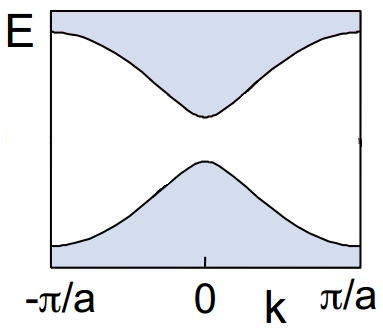
\includegraphics[width=0.5\linewidth]{diagrams/band_insulator_2.png}
				\caption{Free fermion band insulator}
			\end{figure}
			\begin{figure}
			\vskip-0.6cm
				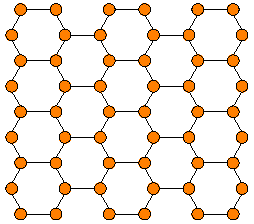
\includegraphics[width=0.5\linewidth]{diagrams/filled_honeycomb.pdf}
				\caption{Atomic picture}
				%Some integer number of localized orbitals filled, integer charge per site
			\end{figure}
		\end{block}
\end{column}
\begin{column}[T]{.5\textwidth}
	\begin{block}{Topological Insulators}
		\vskip-0.3cm
		\begin{figure}
			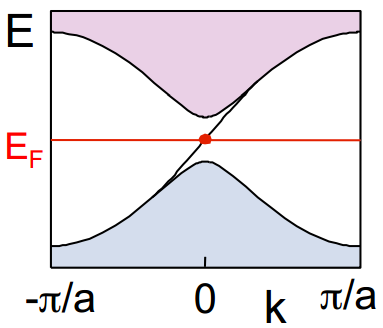
\includegraphics[width=0.5\linewidth]{diagrams/chiral_edge.png}
			\caption{Band insulator with chiral edge \footnotemark}
			%Not viewed as some integer number of orbitals filled per unit cell
		\end{figure}
		\begin{figure}
			\vskip-0.7cm
				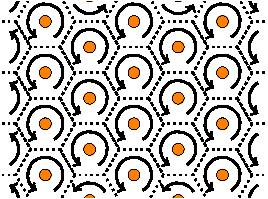
\includegraphics[width=0.5\linewidth]{diagrams/honeycomb_breakdown.pdf}
				\caption{Atomic picture breaks down}
		\end{figure}
	\end{block}

\end{column}
\end{columns}

\footnotetext[1]{
\citep{Hasan2010-fq}}

}
\end{frame}

%Examples include free fermion band insulators, both trivial and topological
%Interacting 1D examples would include the spin-1 heisenberg AFM
\include{slides/theproblem}
\section{Construction of Honeycomb FBI}
\begin{frame}{Construction of 1D Featureless Insulators}
\vskip-1.5cm		
\begin{columns}[T]
	\begin{column}[T]{.5\textwidth}
		\begin{block}{Classical Insulators}
			\vskip0.55cm
			\only<1, 2>{
			\begin{figure}
				
\includegraphics[width=\linewidth] {diagrams/trivial_chain.pdf}
				\caption{1D Trivial Chain}
			\end{figure}
			}
		 \only<3>{
			\begin{figure}
			  \vskip-0.5cm
				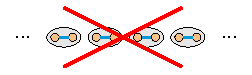
\includegraphics[width=\linewidth] {diagrams/trivial_chain_w_x.pdf}
				\vskip-0.4cm
				\caption{1D Trivial Chain}
			\end{figure}
			}
		\only<2>{
		\bi
		\item[] Product state with one boson per site
		\ei
		}
		\end{block}
	\end{column}
	\begin{column}[T]{.5\textwidth}
		\begin{block}{Topological Insulators}
			\vskip0.45cm
			\begin{figure}
				
\includegraphics[width=\linewidth] {diagrams/haldane_insulator_chain.pdf}
				\caption{1D Topological Chain}
			\end{figure}
		\only<2>{
		\bi
		\item[] Haldane Insulator Phase \cite{pollmann2010}
		\item Unitarily related to AKLT
		\item No $SU(2)$ symmetry
		\item Symmetry protected 2-fold edge degeneracy
		\ei
		}
		\end{block}
	\end{column}
\end{columns}
\only<1>{
\begin{center}
	\begin{figure}[]
		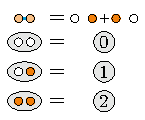
\includegraphics[width=0.4\textheight] {diagrams/haldane_insulator_chain_rules.pdf}
		\caption{Entangled pairs and projectors used in state construction}
	\end{figure}
\end{center}
}
\only<3>{
\begin{center}
	\begin{figure}[]
		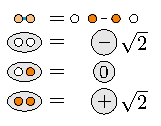
\includegraphics[width=0.4\textheight] {diagrams/aklt_rules.pdf}
		\caption{Entangled pairs and projectors for $SU(2)$ symmetric state}
	\end{figure}
\end{center}
}
\end{frame}

%Examples include free fermion band insulators, both trivial and topological
%Interacting 1D examples would include the spin-1 heisenberg AFM
\begin{frame}{Construction of Honeycomb FBI}
\vskip-1.5cm

\end{frame}
\begin{frame}{Known Results for Honeycomb FBI}
\vskip-1.5cm

\end{frame}
\section{Entanglement Edge of Honeycomb FBI}
\begin{frame}{Tensor Network cut details}
\vskip-1.5cm

\begin{columns}[T]
  \begin{column}[T]{.5\textwidth}
   	    \only<1>{
 	    \begin{figure}
			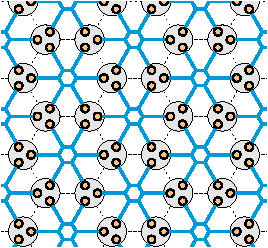
\includegraphics[width=\textwidth]{diagrams/FI_PEPS.pdf}
			\end{figure}
			$$
			\ket{\psi} = \prod\limits_{\varhexagon} \left(\sum\limits_{i \in \varhexagon} b^{\dagger}_i \right) \ket{\mathbf{0}}
			$$ 
		}
  \only<2>{
  		\begin{figure}
			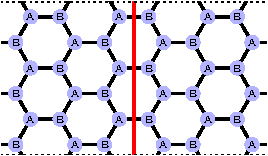
\includegraphics[width=\textwidth]{diagrams/Hex_PEPS.pdf}
			\caption{Generic honeycomb lattice PEPS on zig-zag cylinder with L=3}
		\end{figure}
		}
			\only<3>{
	  		\begin{figure}
			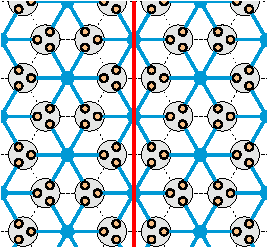
\includegraphics[width=\textwidth]{diagrams/FI_PEPS_wcut.pdf}
			\caption{Honeycomb lattice tensor network on zig-zag cylinder with L=3}
		\end{figure}
	}
\only<4>{
	  		\begin{figure}
			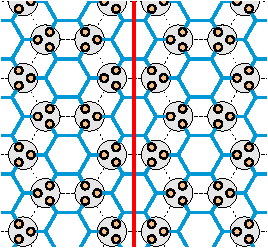
\includegraphics[width=\textwidth]{diagrams/FI_PEPS_wcut2.pdf}
			\caption{Honeycomb lattice PEPS on zig-zag cylinder with L=3, acheived by factoring W-state of plaquette bosons}
		\end{figure}
	}
	\only<5>{
	  		\begin{figure}
			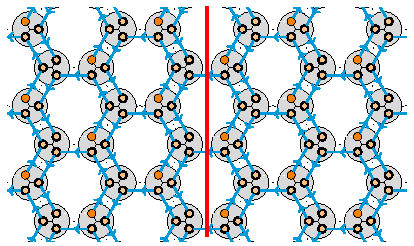
\includegraphics[width=\textwidth]{diagrams/FBI_PEPS_3.pdf}
			\caption{Honeycomb lattice PEPS on zig-zag cylinder with L=3, acheived by factoring W-state of plaquette bosons}
		\end{figure}
	}	
  \end{column}
  \begin{column}[T]{.5\textwidth}
  \vskip0.5cm
       	\only<1>{
     	\begin{figure}
				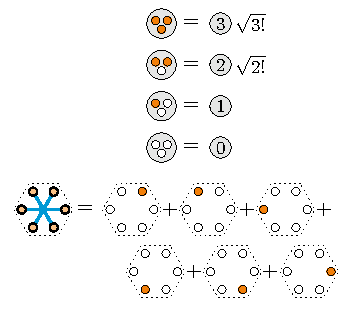
\includegraphics[width=\textwidth]{diagrams/SC_HFBI_rules.pdf}
			\end{figure}
		}
		\only<2->{
  \bi
  \item[] In cylindrical geometry:
  \item Treat state as 1D
  \item Use MPS techniques
  \item On-site translational symmetry parallel to cut
  \item Physical site dimension $4^{2L}$
  \only<4->{
  \item MPS bond dimension = Rank of $\rho_{r}$ =  $2^L$
  \item Entanglement spectrum $\{\epsilon_i\}$ defined from eigenvalues $\{\rho_i\}$ of $\rho_{r}$ via $\epsilon_i = e^{-\rho_i}$
  \item Charge and Translation represented linearly on edge
  }
  \ei
  }
  \end{column}
\end{columns}
\end{frame}
\begin{frame}{Entanglement Spectrum}
\vskip-1.5cm
\only<1>{	
	\begin{figure}[hbctp]
	\begin{center}
	\includegraphics[width=\textwidth]{{EntanglementSpectrum_L10.pdf}}
	%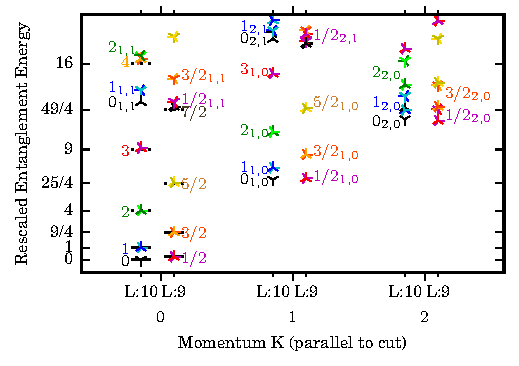
\includegraphics{{interpolatedboson/a10/plots/EEIdentify.pdf}}
	\end{center}
	\end{figure}
}
\only<2>{
	\begin{figure}[hbctp]
	\begin{center}
	\includegraphics[width=\textwidth]{{EntanglementSpectrum_L9.pdf}}
	%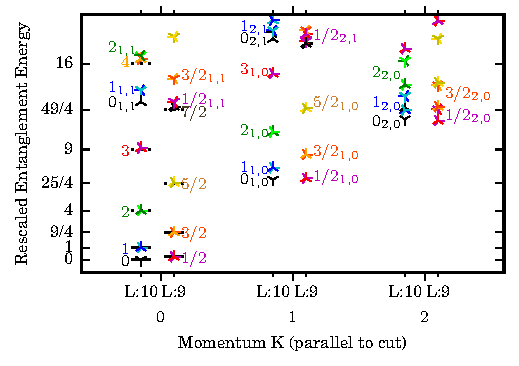
\includegraphics{{interpolatedboson/a10/plots/EEIdentify.pdf}}
	\end{center}
	\end{figure}
}
\end{frame}
\begin{frame}{Finite Size Analysis of Entanglement Spectra}
\vskip-1.5cm
%\begin{columns}[T]
%\begin{column}{.5\textwidth}
\only<1>{
        \begin{figure}[hbctp]
        \centering
        \includegraphics[width=0.8\textwidth]{{EntanglementEnergyScaling.pdf}}
        %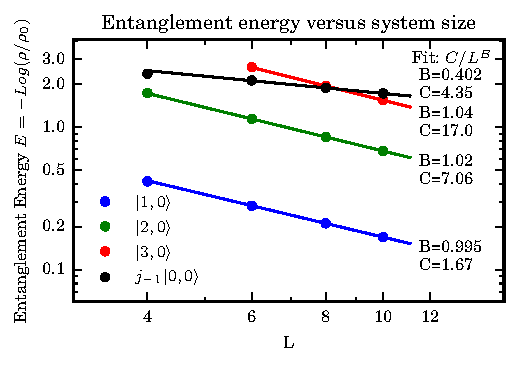
\includegraphics{{interpolatedboson/a10/plots/EntanglementEnergyScaling2.pdf}}
        %\caption{Power law fits for the lowest three states above the ground state at momentum zero and lowest two states at momentum 1 in Figure \ref{fig:sc-EEFinitesize}. The $1/L$ scaling is a signature of a gapless (entanglement) Hamiltonian. The labeling of the states $\ket{e, m}$ or $j_{-1} \ket{e, m}$ is explained in the CFT section below.}
        %\label{fig:sc-EEScaling}
        \end{figure}
%        \bi 
%        \item<1-> Low energy modes show gapless $1/L$ behavior
%        \ei
}
%\end{column}
%\begin{column}{.5\textwidth}
\only<2>{
				\begin{figure}[hbctp]
        \centering
        \includegraphics[width=\textwidth]{{TopologicalEntanglementEntropy.pdf}}
        \end{figure}
}
%\end{column}
%\end{columns}

\end{frame}
\begin{frame}{Identification of Edge CFT}
\vskip-1.5cm
\newcommand{\uL}{\mathbf{L_0}}
\newcommand{\bL}{\mathbf{\bar{L}_0}}

\only<1>{
\begin{block}{Conformal Charge via 'Nested Entanglement Entropy'}
\vskip-0.5cm
	\begin{figure}[hbctp]
	\centering
	\includegraphics[width=0.8\textwidth]{{EdgeGS_EntanglementEntropy.pdf}}
	%\caption{Entanglement entropy within the entanglement ground state of the soft-core boson state on $10$ sites. For comparison, the Cardy-Calabrese formula $S(x) = c/3 \log \sin( \pi x/L) + const.$ is shown with $c=\frac{1}{2}, 1,$ and $2$, with the $const.$ fixed by matching the maximum of the entanglement entropy data. $c=1$ is a good fit.}
	%\label{fig:hc-edge-gs-ee}
	\end{figure}
	\begin{empheq}[box={\mybluebox[4pt][4pt]}]{equation*}
	c = 1
	\end{empheq}
\end{block}
}

\only<2>{
\begin{columns}[T]
\begin{column}{0.35\textwidth}

\begin{block}{Conformal Weights}
We can match the rescaled entanglement energies to the conformal weights of a free bosonic CFT.

%\begin{tabular*}{\columnwidth}{@{\extracolsep{\stretch{1}}}*{2}{c}@{}}
%\begin{tabularx}{\columnwidth}{|X|X|}
%\toprule
%\small
%\begin{align*}
%	\mathbf{P} &=&\frac{2\pi}{L}(\uL-\bL) 
%	&=& \frac{2\pi}{L}(em + n - \bar{n}) \\
%	%\widetilde{\mathbf{P}}&= em + n - \bar{n} &\\ 
%	\mathbf{H} &=& \frac{2\pi}{L}(\uL+\bL) 
%	&=& \frac{2\pi}{L}(\frac{\kappa e^2}{2} + \frac{m^2}{2 \kappa} + \frac{n + %\bar{n}}{2}) %\\
%\end{align*}
%\normalsize

%\begin{empheq}[box={\mybluebox[4pt][4pt]}]{equation*}
%\mathbf{H} \propto e^2 + \frac{m^2}{\kappa^2} + \frac{1}{\kappa}(n + \bar{n})
%\end{empheq}
$$
\mathbf{H} \propto e^2 + \frac{m^2}{\kappa^2} + \frac{1}{\kappa}(n + \bar{n})
$$
\end{block}
%}

%\only<3>{
\end{column}
\begin{column}{0.65\textwidth}
\begin{block}{Conformal primary identification in entanglement spectra}
\begin{figure}[hbctp]
\begin{center}
\includegraphics[width=\textwidth]{{EEIdentify.pdf}}
%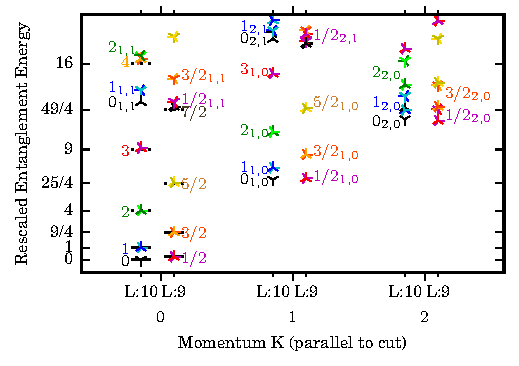
\includegraphics{{interpolatedboson/a10/plots/EEIdentify.pdf}}
\end{center}
%\caption{The identification of the states $\ket{e, m}_{n, \bar{n}}$ in the spectrum of the soft-core boson entanglement Hamiltonian. The label $e$ gives the U(1) charge. The labels $n$, $\bar{n}$ label the levels in the right or left-moving sectors of the Kac-Moody algebra. When the level $n$ is larger than 1, the level shows $Z(n)$ approximately degenerate states. The best estimate for the Luttinger parameter $\kappa = 1/6.4$ is given by the inverse of the energy of the $\ket{1, 0}_{1, 0}$ state. The label $m$ is 0 for all states shown - however, the primary states $\ket{e, m=\pm 1}$ can be seen centered around momentum $\pi$, with energies on the order of $1/(4\kappa^2)$.}
%\label{fig:primaries}
\end{figure}

\end{block}
\end{column}
\end{columns}
}

\end{frame}

\section{Symmetry Protection of Edge}
%!TEX root = ../fbi.tex

\section{Symmetry protection}
\label{sec:symmetry}

\subsection{Overview}

While the gapless entanglement spectrum observed above is consistent with a symmetry-protected
topological phase, it does not by itself guarantee the presence of such a robust phase, and does not
allow us to infer which symmetries are protecting the topological properties of the phase.
A key observation that allows us to make progress on these crucial questions is that many points
in the entanglement spectrum are degenerate. In particular, we find that for cylinders of odd circumference,
the entire spectrum is doubly degenerate.
In this section, we will discuss how
the corresponding degenerate Schmidt states are related through the action of a symmetry of the HFBI wavefunction. 
As discussed in Ref.~\onlinecite{pollmann2010} and reviewed in the Appendix~\ref{Appendix:MPS},
this symmetry action can be used to diagnose one-dimensional symmetry protected topological order,
for which the degeneracy throughout the entire entanglement spectrum is a robust feature.
We will demonstrate that the odd circumference cylinders, considered as quasi-one-dimensional states, 
are indeed SPTs protected by a combination of lattice inversion and charge parity symmetries.

While the Schmidt eigenstates are uniquely defined for non-degenerate eigenvalues of the reduced
density matrix, they are not unique when the spectrum is degenerate and any choice of orthonormal
states in the degenerate subspace represents a valid choice of Schmidt states. Applying
a unitary transformation $V^{ji}$, which respects $\sum_i V^{ji} (V^{ki})^* = \delta_{jk}$, on the
left Schmidt states must be accompanied by an appropriate transformation $(V^{ji})^*$ applied to
the right Schmidt states.

In particular, this allows the action of an on-site symmetry (or more generally, 
any symmetry which commutes separately with the reduced density matrices
for the left and right half) to mix Schmidt states corresponding to degenerate eigenvalues.
The action of such a symmetry operator $U_g$ takes the form
\beq
\label{eq:symschmidt}
\begin{split}
U_g \ket{\psi^{(i)}_{L}} &= \sum\limits_j \ket{\psi^{(j)}_{L}} V_g^{ji} \\
U_g \ket{\psi^{(i)}_{R}} &= \sum\limits_k \ket{\psi^{(k)}_{R}} \left(V_g^{ki} \right)^*,
\end{split}
\eeq
where the $V_g^{ji}$ are unitary matrices that only act on degenerate blocks of Schmidt states.
Crucially, Ref.~\onlinecite{pollmann2010} describes a numerical procedure to calculate $V_g$ for
an on-site symmetry $g$ within the MPS formalism, which we review in Appendix~\ref{Appendix:MPS}.

We can also analyze the effects of symmetries that preserve the entanglement cut but swap
the left and right halves of the cylinders. In general, we will consider 
any symmetry $h$ that swaps the cylinder sides and squares to the identity, which we will call an 
inverting symmetry. These satisfy a modification of~\eqnref{eq:symschmidt}:
\beq
\label{eq:isymschmidt}
\begin{split}
U_{h} \ket{\psi^{(i)}_{L}} &= \sum\limits_j \ket{\psi^{(j)}_{R}} V_{h}^{ji} \\
U_{h} \ket{\psi^{(i)}_{R}} &= \sum\limits_k \ket{\psi^{(k)}_{L}} \left( V_{h}^{ki} \right)^*.
\end{split}
\eeq
Note here that the left and right Schmidt states are exchanged in the transformation. We can
introduce a map $S$ that acts as
\beq
S \ket{\psi^{(i)}_{R}} = \ket{\psi^{(i)}_{L}}.
\eeq
Since a change in phase $\ket{\psi^{(i)}_{R}} \to e^{i \varphi} \ket{\psi^{(i)}_{R}}$ must be
accompanied by the complex conjugate $\ket{\psi^{(i)}_{L}} \to e^{-i \varphi} \ket{\psi^{(i)}_{L}}$
to preserve the Schmidt decomposition, $S$ is antiunitary.

Combining the above, we see that
\beq
\label{eq:isymschmidt2}
U_h S \ket{\psi^{(i)}_{R}} = \sum\limits_j \ket{\psi^{(j)}_{R}} V_{h}^{ji}
\eeq
defines the action of the operator $U_h S$ on the right Schmidt states (of course an equivalent
action can be defined on the left Schmidt states). Since $S$ is anti-unitary, the combined action
of $U_h S$ is also anti-unitary.
Together with the requirement that the symmetry squares to the identity, one finds that
(where $\mathbf{K}$ represents complex conjugation in the canonical basis)
\begin{equation}
V_h V_h^* = (V_h \mathbf{K})^2 = e^{i \phi_h} I = \pm I,
\end{equation}
that is the inverting symmetry forms an anti-unitary projective representation of $\mathbb{Z}_2$.

As reviewed in Appendix~\ref{Appendix:MPS}, the collection of $V_g$ of on-site symmetries 
sometimes fail to satisfy the group multiplication laws, i.e. one may find $V_{g_1 g_2} \neq V_{g_1} V_{g_2}$.
Instead, they may form a projective representation, where group multiplication laws are obeyed up
to phases $\omega(g_1, g_2)$, i.e. $V_{g_1} V_{g_2} = \omega(g_1, g_2) V_{g_1 g_2}$.
The equivalence classes of $\omega(g_1, g_2)$ are classified by the elements of $H^2(G, U(1))$. 
If the element is non-trivial, i.e. there exist $g_1$, $g_2$ such that $\omega(g_1,g_2) \neq 1$,
the degeneracy in the entanglement spectrum on which $V_g$ acts cannot be removed
without breaking the symmetry, since the distinct classes of $H^2(G, U(1))$ cannot be
connected continuously. \bela{This is not obvious and needs a citation.}
Similarly, for the inverting (anti-unitary) symmetries $h$, the phase $\phi_h = -1$ signifies that 
the degeneracy cannot be removed without breaking the symmetry.\cite{pollmann2010}.

\subsection{Symmetry protection of the HFBI}

The on-site symmetries of the featureless boson insulator considered here
are the $U(1)$ charge symmetry and the 
anti-unitary symmetry $\tau$, which acts by complex conjugation in the boson number basis.
Despite being at half-filling, the hard-core boson variant of the state does not have a particle-hole
symmetry. Exploring the edge action of these symmetries numerically, we find that they are all
represented linearly and thus do not protect the degeneracy of the entanglement spectrum
on cylinders of odd circumference.
In order to protect the degeneracy, we must therefore include lattice symmetries.

%In the cylinder geometry chosen, the group of lattice symmetries consists of translations 
%- generated by $T_x$ parallel and $T_y$ perpendicular to the cylinder axis-
%as well as reflections $\I_x$ through a line parallel 
%and $\I_y$ through a line perpendicular to the cylinder axis. 
%We also consider lattice inversion $\I = \I_x \I_y$, equivalent to a $\pi$ 
%rotation of the spatial plane about the center of a hexagonal plaquette.
By choosing a cylinder geometry, we explicitly break some of the lattice rotational
and reflection symmetries. In this case, we will only need the lattice inversion $\I$,
a $\pi$ rotation of the spatial plane about the center of a hexagonal plaquette. 
By analysing Equation~\ref{eq:isymschmidt2}, one sees that $V_{\I}$ will map each Schmidt 
state to a state with the same entanglement energy and momentum, but with opposite charge -
since $U_{\I}$ flips momentum, but the Schmidt pairing $S$ pairs each state with a state of
opposite charge and momentum. 
Thus $V_{\I}$ swaps the degenerate pairs of states $\ket{e, m; n, \bar{n}}$ and
$\ket{-e, -m; \bar{n}, n}$ which appear in Figure~\ref{fig:ESL910}. 

Our numerical results show that 
$$
V_{\I} V_{\I}^* = I, 
$$
so inversion alone does not protect the degeneracy. Instead, we find that the
combined symmetry $\varPi \mathcal{I}$ protects the degeneracy:
$$
V_{\varPi \I} V_{\varPi \I}^* = -I 
$$
where $\varPi = e^{i \pi \mathcal{Q}} \in U(1)$ is the charge parity symmetry.
This can be understood simply. For odd $W$, where the charges $e$ are half-integer,
states with opposite charge $e$ and $-e$ also differ in charge parity. $V_{\varPi}$
acts with a relative phase between these states. Thus, if $V_{\I}$ squares
to $I$, $V_{\varPi \I}$ squares to $-I$, and vice versa.  
It is easy to produce a variant on the HFBI state with the opposite situation where
the roles of $\I$ and $\varPi \I$ are switched - this is discussed further in 
Appendix~\ref{Appendix:Variants}.

\brayden{What do you think of this discussion?}
In the next section, we will discuss the consequences of this 1D symmetry protection 
for perturbations of a quasi-local parent Hamiltonian. Most importantly, it tells us
that the edge physics is not finely tuned but survives perturbations that respect the
protecting symmetry; specifically, perturbations of the Hamiltonian that 
remain on the honeycomb lattice,
are invariant under $\varPi \I$,
and have unique ground states on odd $W$ cylinders
will also show the degenerate entanglement spectrum in their ground states.
These conditions are enough to show that the state is a 2D SPT - that is, 
it cannot be adiabatically connected to a product state - when both $\varPi \I$ and
the translationally symmetry group of the lattice are preserved. Not breaking the
translational symmetry group is necessary for the argument to go through, since spontaneous
translational symmetry breaking leads to states that do not have unique ground states
on odd $W$ cylinders - and explicit breaking of translational symmetry, say by adding sites
off the honeycomb lattice, can blur the distinction between odd and even $W$ cylinders.
On the other hand, this symmetry protection does not allow us to guarantee the thermodynamic
degeneracy of the entanglement spectrum - such as a gapless entanglement edge - for regions
that don't wrap around the cylinder or on even cylinder sizes. If a gapped and 2D local 
parent Hamiltonian can be found, it is likely that arbitrary shaped entanglement cuts
must show entanglement features if enough symmetry is protected - but the topological invariant 
given is not enough evidence for that, and it is not clear how much symmetry will be needed.

%Using the techniques of MPS, we can find a quasi-local parent Hamiltonian for a given
%fixed cylinder width $W$ that acts on neighboring cylinder slices. By adding perturbations
%to this Hamiltonian on a cylinder with $W=3$, we can check that the degeneracy of the
%entanglement spectrum does not get split even when charge and translational
%symmetry are explicitly broken, as long as $\varPi \I$ is unbroken. In addition, this
%symmetry protection implies a non-local string order parameter that detects this phase.

There is also a second symmetry group that can protect the entanglement degeneracy.
Since $V_{\tau}$ and $V_{\I}$ acts antiunitarily, one can show that $V_{\tau \I}$ acts
unitarily on the edge. The $\mathbb{Z}_2 \times \mathbb{Z}_2$ group generated by
$\tau \I$ and $\varPi$ has a projective representation characterized by the 
topological invariant
\beq
V_{\varPi} V_{\tau \I} V_{\varPi}^{-1} V_{\tau \I}^{-1}
 = - I.
\eeq
This symmetry protection gives a distinct class of perturbations that cannot
split the entanglement degeneracy for odd $W$.


\begin{tabular*}{\columnwidth}{@{\extracolsep{\stretch{1}}}*{6}{r}@{}}
\toprule
$\mathbf{G}$ & i & Q & K & $\mathbf{\theta_g}$ & $\mathbf{\phi_g}$ \\
\midrule
 $Id            $ & + & + & + & + & + \\
 $\varPi        $ & + & + & + & - & + \\
 $\I            $ & - & - & + & + & + \\
 $\tau          $ & - & + & - & + & + \\
 $\varPi \I     $ & - & - & + & - & - \\
 $\varPi \tau   $ & - & + & - & - & + \\
 $\tau \I       $ & + & - & - & + & + \\
 $\varPi \tau \I$ & + & - & - & - & - \\
\bottomrule
\end{tabular*}



%However, the entanglement spectrum of this one wavefunction is not enough to
%determine the SPT nature of the phase. First, it isn't clear what group or
%groups of symmetries can be used to protect the gapless edge. It could be that
%the entire symmetry group - $U(1)$ boson number conservation, \brayden{time
%reversal symmetry?}, as well as the entire rotational and translational group
%of the lattice - must be preserved to protect the edge. Or, as we will argue
%is the case, a much smaller subgroup could be used to protect the edge. This
%leads to a wider class of perturbations that leave the edge intact - and since
%we will argue that translation is not needed for protection, the gapless edge should additonally be robust to some types of weak disorder and can be seen in
%small systems with symmetry preserving boundary conditions. Second, the
%entanglement spectrum alone fails to distinguish between other SPT phases with
%the same protecting group - for that, we need a topological invariant. Third,
%we would like to confirm the SPT nature of the phase by perturbing a parent
%Hamiltonian with terms that break various combinations of symmetries and
%seeing if they destroy the gapless edge.

%To determine the protecting group, we can proceed in
%two ways: we could perturb a parent Hamiltonian with terms that break various
%combinations of symmetries and see which perturbations destroy the gapless
%edge, or we can look for a topological invariant by analyzing the action of
%the symmetry of the entanglement edge. We will take up the later question
%first, then return to the prospect of perturbing a parent Hamiltonian in
%Section \ref{sec:perturbations}.


%Given that only odd circumference cylinders are SPTs, one might wonder whether
%odd and even $L$ cylinders approach two differt phases in the thermodynamic
%limit. In Section~\ref{sec:CFT}, we will provide evidence against that
%possibility, by showing that in both cases, the low-energy, linear dispersing
%part of the entanglement spectra can be described by the same conformal field
%theory. Thus, in the thermodynamic limit, the two edge spectra approach the
%same set of points.
\begin{frame}{Future Work}
\vskip-2cm

\begin{columns}[T]
    \begin{column}[T]{.9\textwidth}

\begin{block}{}
	\bi
	\item[] Entanglement properties with different geometries
		%Which entanglement cuts have exact spectrum degeneracy 
		%Which cuts give you a gapless mode in thermodynamic limit
		\bi
		\item Armchair cylinder edge %Preliminary results suggest
		\item Finite size clusters 
		\item Explain results for arbitrary geometries with tensor network properties, e.g. 'MPO injectivity'
		\ei
	\item[] Find a 2D local Hamiltonian and confirm with numerics
	
		\item[] \vskip-0.5cm $$H_{EBH} = \left(\sum\limits_{\varhexagon} \sum\limits_{i,j \in \varhexagon} -t b^{\dagger}_i b_j + V n_i n_j \right) +\mu N ?$$ 
	\item[] Physical properties of the phase
	\item[] Can we construct% or find obstruction to
	 an SU(2) symmetric FI?
	\ei	
\end{block}

    \end{column}
    \begin{column}[T]{.1\textwidth}
    \end{column}
\end{columns}
\end{frame}
\section*{}
\frame{
  \vspace{2cm}
  {\huge Questions?}

  \vspace{3cm}
  \begin{flushright}
    Brayden Ware

    \structure{\footnotesize{brayden@physics.ucsb.edu}}
  \end{flushright}
}

\frame{
  \vfill
  \centering
  \highlighton{
  \usebeamerfont*{frametitle}Bonus slides

  %\usebeamerfont*{framesubtitle}Bonus slides
  }
  \vfill
}

\begin{frame}
  \frametitle{Resources}
  \vskip-1.7cm
  %\framesubtitle{If you want to improve this style}
  \bibliography{references}
  %\beamertemplatearticlebibitems
\end{frame}


\end{document}
